%\documentclass[useAMS,usenatbib,10pt]{article}
%\documentclass[a4paper,12pt]{article}
\documentclass[useAMS,usenatbib]{mn2e}
\usepackage{graphicx}
\usepackage{fixltx2e}
\usepackage{subfigure}
\usepackage{times}
\usepackage{amsmath}
\usepackage{amsfonts}
\usepackage{url}
\usepackage{placeins}
\usepackage{natbib}
\usepackage{amssymb,amsmath}
\usepackage[normalem]{ulem}
\usepackage{soul}
\usepackage{lipsum}
\usepackage{longtable}
\usepackage{pdflscape}
\usepackage{amsmath}
\usepackage{multirow}
\usepackage{booktabs}
\newcommand{\et}{et al.}
\newcommand{\hmpc}{h^{-1}\,\rm Mpc}
\newcommand{\hkpc}{h^{-1}\,\rm kpc}
\usepackage{lipsum}


\begin{document}
%latex HODpaper_v2.tex ; bibtex HODpaper_v2 ; latex HODpaper_v2.tex ;  latex HODpaper_v2.tex ;dvips HODpaper_v2.dvi ; ps2pdf HODpaper_v2.ps

\title[Quasar HOD at $z \sim 1.5$]{A Halo Occupation Interpretation Of Quasars At $z\sim1.5$ Using Very Small Scale Clustering Information}
% done like the title--> suggestions?
% 
\author[Eftekharzadeh et al.]{S. Eftekharzadeh$^{1,2}$,  A. D. Myers$^{1}$, E. Kourkchi$^{3}$, et al.\\
\\
$^{1}$ Department of Physics and Astronomy, University of Wyoming, 1000 University Ave., Laramie, WY 82071\\
$^{2}$ Department of Physics, Southern Methodist University, 3215 Daniel Ave., Dallas, TX 75225\\
$^{3}$ Institute for Astronomy, University of Hawaii, 2680 Woodlawn Drive, Honolulu, HI 96822, USA}
\maketitle


\begin{abstract}
We couple the most accurate small scale ($< 100\, \rm h^{-1}kpc$) quasar clustering 
to date with its most recent counterpart at large scale ($> 1\, \rm h^{-1}Mpc$) 
from the extended Baryon Oscillation Spectroscopic survey (eBOSS) in an attempt 
to better constrain the satellite fraction of quasars at $z\sim 1.5$ as one of the more controversial 
parameters of structure formation hierarchy in the halo occupation framework. 
We built our Halo Occupation Distribution (HOD) framework based on commonly 
used analytic forms for the one and two-halo terms with the two free 
parameters: the minimum halo mass that host a central quasar and the fraction of satellite quasars and within one halo. 
%We investigated the effect of relaxing the width of the halo mass distribution as the third parameter to the model and found it to have no significance in the best-fit model.
Inspired by the latest studies that proposed a steeper density profile for the dark 
matter haloes to recover the observed excess clustering at kiloparsec scales, we 
explored the change in the model and the best-fit parameters for a range of 
concentrations. We found that an HOD model with a satellite fraction of $f_{\rm 
sat} = 0.062_{-0.026}^{+0.018}$ and minimum mass of $\rm M_{m} = 
2.316_{-0.440}^{+0.463} \times 10^{12}\, \, \rm h^{-1} M_{\odot}$ for the host dark matter 
haloes would best describe the {\it full} quasar clustering at $z \sim 1.5$. Our derived satellite fraction is consistent with recently reported value for 
quasars at $z\sim 1.4$ that uses the same HOD formalism. Our findings could be interpreted as an evidence that the commonly used parameterization for the mean number of quasars in each 
halo is unable to further characterize the halo occupation distribution of 
quasars.   
% $\Delta_{\rm m}= 0.741_{+0.149}^{-0.208}$



\end{abstract}

 \begin{keywords}
 cosmology: observations, small-scale clustering, halo occupation; quasars: general, surveys, close pairs
 \end{keywords}

\section{Introduction}
\label{intro}
The advent of the first large, homogeneous surveys of the extragalactic sky prompted
cosmologists to begin to think about galaxies as discrete points embedded in 
statistical structures \citep[e.g.][]{nsz62,ns74}. These structures could
be characterized in terms of their size, the distribution of the discrete points
that occupied them, and their distribution across the wider Universe
 \citep[see, e.g. ][for a review]{cs02}. As it became increasingly clear
 that dark matter dominated the mass budget in galaxies \citep[e.g.][]{Roo72,Ost74,Rub78}, it became more natural
 to think of occupation statistics in terms of the virialized haloes that host 
 luminous tracers \citep[e.g.][]{Whi78}.
This line of reasoning ultimately led to empirical approaches that describe how 
cosmological tracers occupy underlying dark matter structures, such as the Halo 
Occupation Distribution framework \citep[HOD; e.g., ][and references therein]{bw02,zh07}.
Parameterizations of the HOD typically consist of of a two-halo term, which characterizes how haloes of a certain
mass cluster around each other, and a one-halo term that relates galaxy and dark matter statistics through the
probability that a halo of a given mass contains a number of galaxies of a given
type. 

The key observables that are used for constraining HOD descriptions in the common formalism
are the number density and the clustering of a given tracer population. 
As such, the HOD framework has now been successfully used to model galaxy
clustering measurements for a wide range of redshifts and galaxy
types \citep[e.g.,][]{2dFsurv,daw16}
%{AddAHalfADozenOrSoReferencesHereFor2dF,SDSS,eBOSS,etc}.   ------------> SE: don't know which ones
Quasars, the most luminous of the Active Galactic Nuclei, are driven by accreting
supermassive black holes at the centers of galaxies. It is now well-established that the centers of most galaxies 
contain a supermassive black hole \citep[e.g.][]{Kor95}, and that the evolution of active quasars and inactive 
galaxies is interrelated \citep[e.g.][]{Kau00}. It is therefore reasonable to think of quasars simply as a biased tracer
of certain types of galaxies that should also, in theory, be empirically describable using HOD statistics.

In the wake of large spectroscopic surveys of quasars such as the 2dF \citep[][]{2dFsurv} and SDSS 
\citep[e.g.,][]{fu96,gu98,yo00,va01,st02,str02,te04,we04,yi04a,yi04b,bo04,ro05,wi05}, the clustering of quasars has been measured at a range of redshifts
\citep[e.g.,][]{cr04,po04,my06,my07,my07b,she07,she09a,ro09,ric12,wh12,ric13,ro13,ef15,la17}.
Typically, these studies focus on the large-scale clustering of quasars via the two-point correlation function, which 
constrains the ``two-halo term'' that describes how ``central'' dark matter haloes cluster around each other. The consensus is that, 
at most redshifts, quasars occupy central haloes of masses a few times $10^{12}\,h^{-1} {\rm M_{\odot}}$. 

Probing how quasars are distributed within haloes---the so-called ``one-halo'' term---is trickier, however. As 
quasars occupy massive haloes, they are rare in general. Further, the haloes that host quasars, particularly at 
high redshift \citep[e.g.,][]{wh12,ef15}, are on the steeply falling part of the halo mass function.% \cite[][]{BeNiceToAddAReferenceHere}. % SE: I'll have to look them up more ... havent found any yet
This implies that instances of two quasars occupying a single halo at high redshift may be very rare indeed. 
Finding close pairs of quasars is complicated further by the fact that most large spectroscopic surveys use 
fiber-fed multi-object spectrographs. Such surveys can have restrictions on how closely fibers can be placed 
together on the sky, which has prompted follow-up surveys of close quasar pairs using long-slit spectrographs 
\citep[e.g.,][]{Hen06,my08,Hen10,ko12,ef17}. These long-slit surveys, in combination with the large-scale two-point
correlation function, have been used to constrain the one-halo term for quasars via clustering measurements over 
a wide redshift range of redshift ($z \sim$ 0.5--3) and scale \citep[][]{ric12,ko12,sh13}.

Recent measurements of quasar clustering have used a number of different assumptions for the overall form
of the quasar HOD. For instance, KO12 model both the distribution of satellite and
central quasars using Gaussians, ultimately expressing the HOD using two-to-three fitting  
parameters. On the other hand, \citet{zh07,ric12,ric13,sh13} use a model that combines a power-law with
a Gaussian, which requires five-to-six fitting parameters. These choices, however, seem to have little
power to constrain the one-halo term of the quasar HOD as KO12 and \citep{sh13} derive consistent 
satellite fractions using their two different HOD parameterizations. Much of this degeneracy regarding the form of the quasar 
HOD is driven by sizable uncertainties in the parameters that are fit to model quasar clustering on small scales. It is likely, 
then, that much larger samples of quasar pairs with small separations, or alternative approaches to deriving the 
Mean Occupation Function of quasars \citep[e.g][]{Cha13}, will be needed to probe the overall statistics of how
quasars occupy individual haloes.

Despite the range of possible forms for the Mean Occupation Function of quasars, it remains important to provide empirical 
constraints on the quasar HOD. Large surveys such as the {\em extended Baryon Oscillation Spectroscopic Survey} 
\citep{my15,daw16} and surveys with the {\em Dark Energy Spectroscopic Instrument} \citep{DESI1,DESI2} are beginning to use 
quasars to constrain the cosmological world model at moderate redshift via redshift-space distortions and the Baryon 
Acoustic Oscillation scale. Sophisticated simulations are required to model these cosmological constraints, which require 
an assumed form for the quasar HOD on small scales \citep[e.g.][]{rod17}. Recently, we assembled by far the largest sample of 
quasar pairs that can be used to probe quasar clustering on scales of a few dozen kiloparsecs, well into the one-halo 
regime \citep[][]{ef17}. In this paper, we combine the sample of \citet{ef17} with other clustering results on larger 
scales \citep[e.g.][]{ko12,la17} to provide the best current constraints on the quasar HOD.




This paper is structured as follows: $\S$\ref{dat} summarizes the properties of 
the samples that are used in small and large scale clustering measurements. The measurements 
themselves are detailed in $\S$\ref{cls}, the modeling approach and the chosen 
parameterization is described in $\S$\ref{hodmod}, and 

We adopt a $\Lambda$CDM cosmological model 
with matter and dark energy and baryon density densities of $\Omega_{m}=0.308$, 
$\Omega_{\Lambda}=0.693$, and $\Omega_{b}=0.045$ the Hubble parameter $h=0.678$, 
amplitude of matter fluctuations $\sigma_{8}=0.814$, and the slope of the 
initial power spectrum $n_s=0.968$ consistent with 
\citet{planck15}. All distances quoted throughout the paper are in comoving 
coordinates unless noted otherwise, denoting the proper coordinates with addition of ``p'' to the distance units (i.e., $ \rm h^{-1}pkpc$ or $ \rm h^{-1}pMpc$). 
\begin{figure*}
    \centering
    \begin{subfigure}{
        \centering
        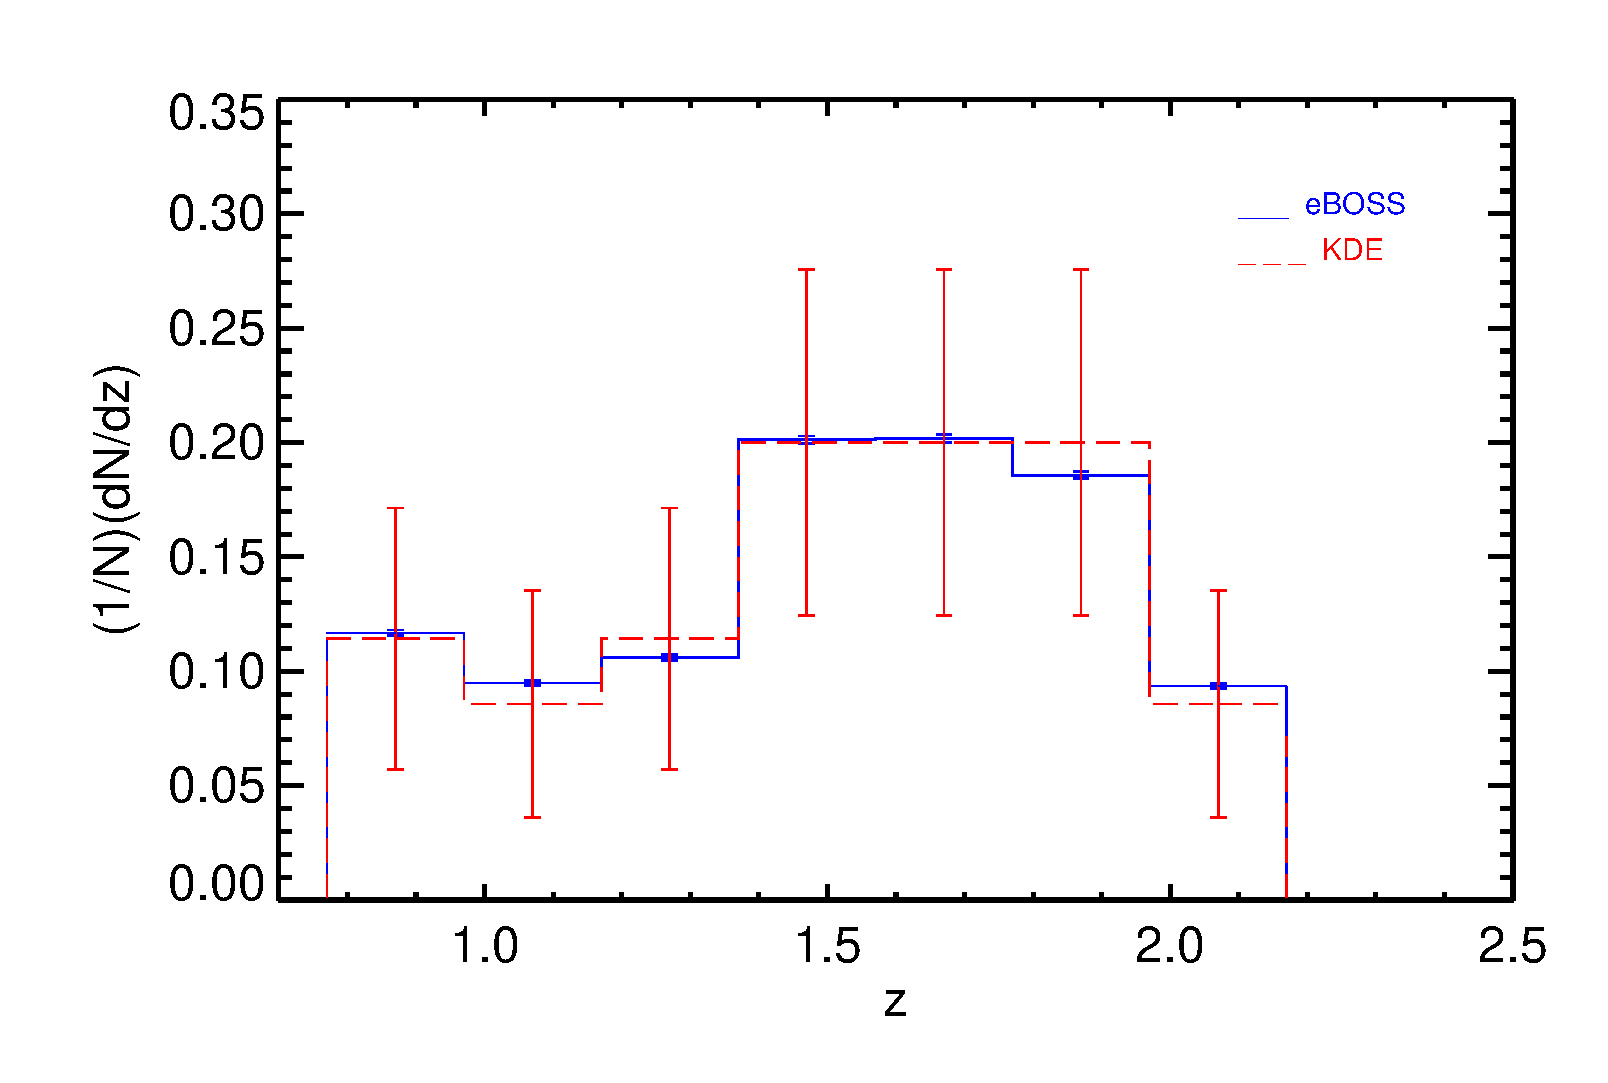
\includegraphics[angle=0,scale=0.29]{NEWmatched_Nz.eps}
        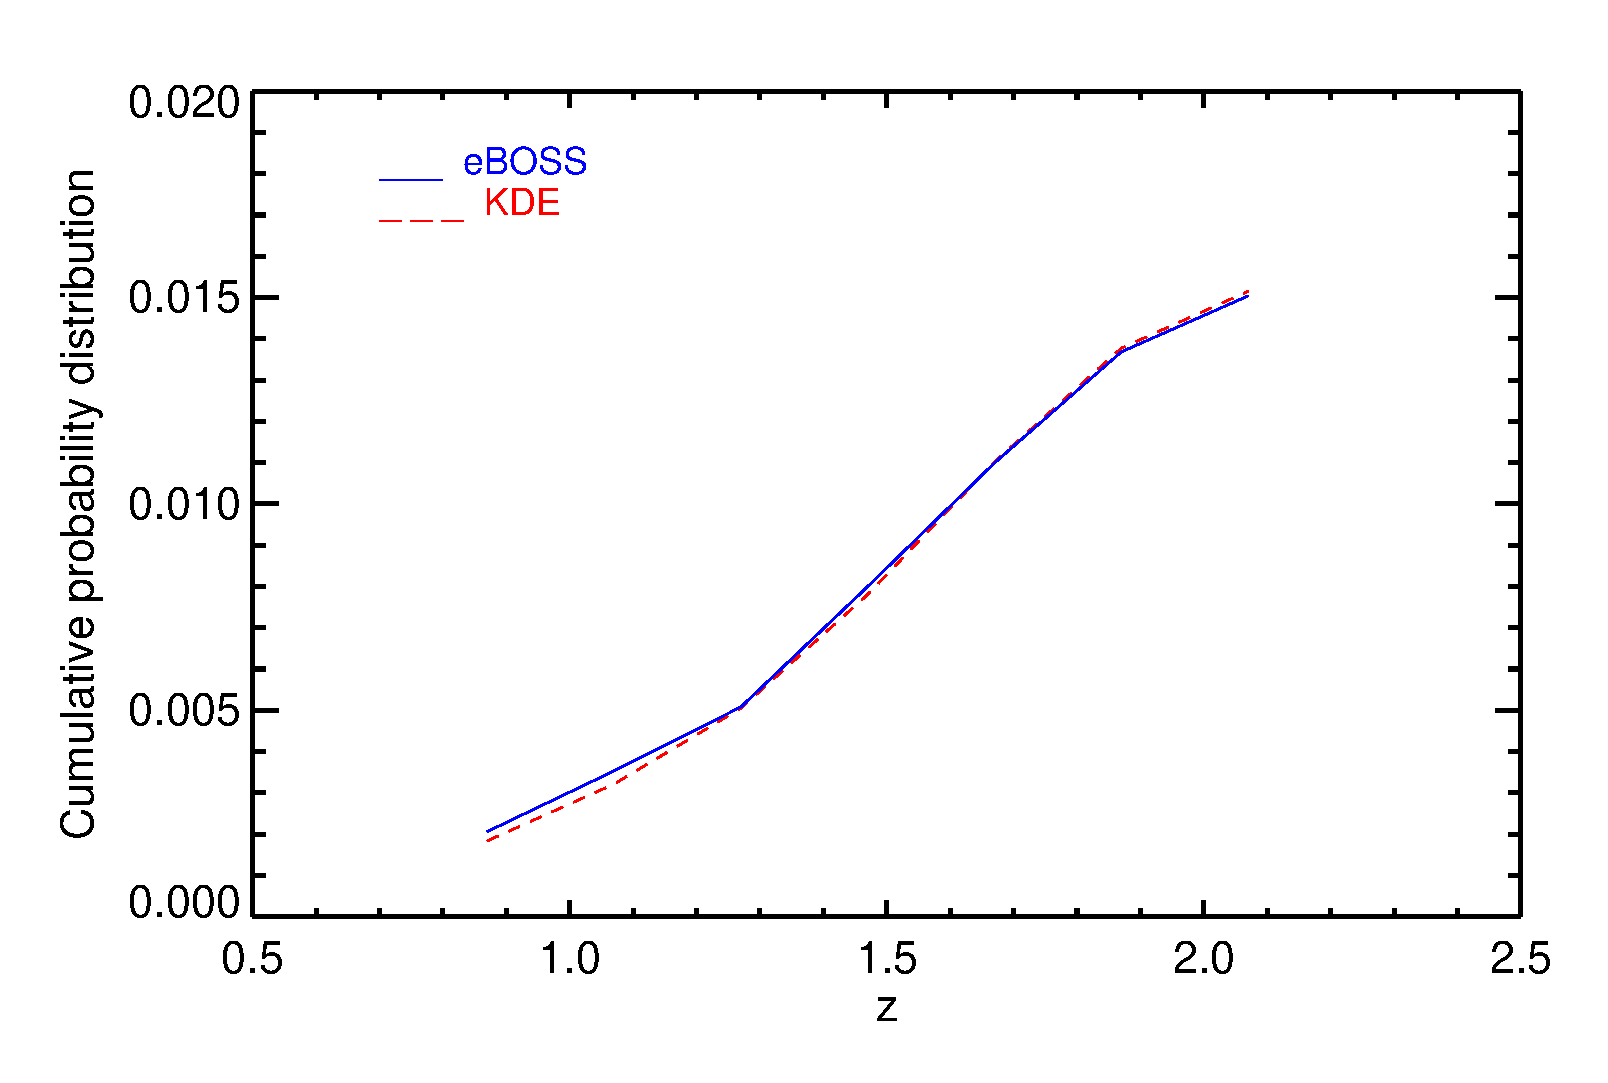
\includegraphics[angle=0,scale=0.29]{KDE_geBOSS_CDFs.eps}}
        \caption{Right: Normalized redshift distribution of the KDE-complete sample of ($<7 \arcsec$) pairs in dashed red and the ``downsampled'' redshift distribution of the eBOSS quasars in solid blue. The ``down sampling'' process was performed due to the need to match the redshift distribution of the eBOSS quasars to be able to use their co-joint clustering measurements for a halo occupation interpretation (see $\S$\ref{dat}). Left: the cumulative distribution function (CDF) of KDE and eBOSS samples. The Kolmogorov-Smirnov test shows that the probability that these two samples are drawn from the same distribution is $86\%$.} \label{fig1:nz-cdf}
        \end{subfigure}


\end{figure*}

\begin{table*}
\centering
\begin{tabular}{cccccccc}

\hline
\hline
$z_{min}$   &$z_{mid}$ &$z_{max}$& $(1/N_{eBOSS})~dN/dz$ & Error & $(1/N_{KDE})~dN/dz$& Error\\

\hline


0.77 & 0.87 & 0.97 & 0.117 & 0.001 & 0.114 & 0.057 \\
0.97 & 1.07 & 1.17 & 0.095 & 0.001 & 0.086 & 0.049 \\
1.17 & 1.27 & 1.37 & 0.106 & 0.001 & 0.114 & 0.057 \\
1.37 & 1.47 & 1.57 & 0.201 & 0.002 & 0.200 & 0.076 \\
1.58 & 1.67 & 1.77 & 0.202 & 0.002 & 0.200 & 0.076 \\
1.77 & 1.87 & 1.97 & 0.186 & 0.002 & 0.200 & 0.076 \\
1.97 & 2.07 & 2.17 & 0.094 & 0.001 & 0.086 & 0.049 \\

\hline
\end{tabular}
\caption{ Normalized distribution of the spectroscopic redshifts of quasars in eBOSS (4th column) and the KDE-complete sample of close pairs (6th column) in the bins of redshifts depicted in Fig.\,\ref{fig1:nz-cdf}.}\label{tab:dndz}

\end{table*}

\begin{figure*}
    \centering
    \begin{subfigure}{
        \centering
        \includegraphics[angle=0,scale=0.27]{gmag_R_theta_eBOSS_KDE.eps}
        \includegraphics[angle=0,scale=0.27]{z_R_theta_eBOSS_KDE.eps}}
        \caption{Angular separation of quasars in each of the pairs that are 
used for the small and large-scale clustering measurement as a function of their 
g-magnitudes (left) and their redshifts (right). Blue dots and green circles in 
the left and orange dots and pink circles in right each represent one pair of 
two confirmed quasars. The open circles in both panels represent the 44 ($< 7 
\arcsec$) pairs drawn from a KDE-complete ``parent sample'' of  243{,}110 quasar 
candidates (see \citet{ef17} for detail). The blue and orange dots in left and 
right panels are the quasar pairs in a sample of 39{,}083 $g\le 20.85$ quasars 
from eBOSS. For consistency, we applied the same magnitude and redshift limits to both samples. 
As is shown, both set of pairs from the small and large angular separations 
exhibit similar distributions in magnitude and redshift. 
The angular separations of the pair members are translated into the 
comoving transverse separation at the average redshift of both samples ($z\sim 
1.5$) and shown on the top axis of both panels. Fiber collision of multi-fiber 
spectrographs in eBOSS (and BOSS), imposes a lower limit of $62\arcsec$ for the 
angular separation of the quasar pairs, causing a $\sim 55\arcsec$ gap between 
the close pairs from the KDE-complete sample at $7\arcsec$ and the eBOSS 
pairs.}\label{fig2:gz}
    \end{subfigure}
\end{figure*}



\section{Data}\label{dat}
 We used two independently compiled samples of confirmed quasars for clustering 
measurements at kpc and Mpc scales. The small scale clustering measurement used in this work is drawn from a complete sample of 
$g<20.85$ confirmed quasars at $z \sim 1.5$ and the large scale clustering measurement is 
made using a sample of $g<20.85$ quasars from the extended Baryon 
Oscillation Spectroscopic Survey \citep[eBOSS; DR14][]{daw16,dr14} at similar average redshift. We applied a number of adjustments prior to measuring the two-point correlation function and combining these two measurements into one that spans over comoving distances of $\sim 0.01-100 \, \rm h^{-1}Mpc$. The goal has been to combine these two measurements to be used in our halo occupation interpretation. In the following, we summarize the compilation process and properties of the two samples.

\subsection{KDE-complete sample of close pairs and the associated random catalog}\label{sdat}
The basis for the follow up spectroscopy that led to the complete sample of 47 spectroscopically confirmed ``binaries'' with the angular separation of $2.9\arcsec \leq \theta \leq 7.7\arcsec$ at $0.43 \leq z \leq 2.2$ is a sample of 1{,}172{,}157 high probability quasar candidate drawn via a Kernel Density Estimation technique \citep[KDE;][]{ric04} on all the point sources in SDSS-DR6\citep[][]{admc08} imaging data down to $i=21.3$. A total of 290{,}694 quasar candidates at $0.43 \leq z \leq 2.2$ were selected via a non-parametric Bayesian classifier with $\sim 92.7\%$ efficiency \citep[see ][and references therein for detail]{ef17}. A carefully designed long-slit spectroscopy campaign observed a homogeneous subsample of these pair candidates over the course of three years \citep[see Table 1 of ][for detail]{ef17}. 

Out of the 47 pairs in the KDE-complete sample \citep[presented in Figure 4 and Table 5 of][]{ef17}, 44 reside in the selected redshift range for this study ($0.8 \lesssim z \lesssim 2.2$ with $\bar z\sim 1.5$). The comoving separations of quasars in these pairs span over $43.3 \lesssim r_p \lesssim 92.3 \, \rm h^{-1}kpc$. This sample constitutes is used for our sub-Mpc clustering measurement. We later discuss combining our small-scale measurement with a previous measurement at a similar average redshift by \citet{ko12} (hereafter KO12) to fill-in the gap between the last bin of small-scale (at $\sim 85 \, \rm h^{-1}kpc$) of the measured correlation function at small and large scales (see \S\ref{cls}). 

Following the same procedure for calculating the number of ``expected'' quasar-random pairs ($\langle QR \rangle = N_{\rm Q}/N_{\rm R} \times QR$), we construct the random catalog by populating a circular polygon with angular radius of $7.7\arcsec$ around each of the 243{,}110 of quasar candidates \citep[see section 3.1 of][for a detailed description of the taken steps for constructing the random catalog]{ef17}. 


\subsection{eBOSS quasars with $g<20.85$ and the associated random catalog}\label{ldat}

For Mpc-scale clustering measurement, we used a large sample of spectroscopically confirmed quasars from the extended Baryon Oscillation Spectroscopic Survey \citep[eBOSS;][]{daw16} that aims to extend BAO studies to higher redshifts by measuring the redshift for about 0.5 million quasars at $0.8\lesssim z \lesssim 2.2$ as well as $\rm Ly\alpha$ forest quasars at $z>2.1$, luminous red galaxies at $0.6<z<1.0$, emission line galaxies at $z>0.6$ \citep[see ][for target selection criteria and process]{my15}. In order to reduce the risk of missing targets by the target selection algorithm, eBOSS corrects for variance of the $5-\sigma$ detection limit for the photometrically identified point sources across the survey footprint and for different bands. The correction includes applying a depth-dependence systematic weight, $w_{sys}:$ {\tt WEIGHT\_SYSTOT}, to each quasar as well as considering redshift failure ($w_{zf}:$ {\tt WEIGHT\_NOZ}) and fiber collision ($w_{cp}:$ {\tt WEIGHT\_CP}) weights \citep[see, ][for detail of the weight determination]{la17,rod17,bp17,an12,ross12}. The total weight for each quasar is therefore defined as $w_{qso} = w_{\sc fkp}w_{sys}(w_{zf}+w_{cp}-1)$ where $w_{\sc fkp}:$ ({\tt WEIGHT\_FKP  }) is the applied weight for optimum estimation of the two point correlation function \citep[see, ][]{fkp94}.


As eBOSS utilizes the same fiber-fed optical spectrograph as BOSS, the fibers can not get closer than $62 \arcsec$ in the spectroscopic plates except for the overlapping regions\citep{bl03}. This angular separation limit is equivalent to the comoving separation of $0.37\, \rm h^{-1}Mpc$ at $z\sim 1.5$. For clustering measurement at small scales, it is more important to be complete as the interplay between the fiber collision radius and the {\it unknown} small-scale clustering of the targets is impossible to perfectly reconstruct. Although quasar samples are sparse enough that the number of collided pairs is very small \citep[e.g.,][]{rod17}, we set the first bin of comoving separation at which we started to measure the two-point correlation function (2PCF), to be at $1.1 \, \rm h^{-1}Mpc$ \citep[see, e. g., ][for studies on the efficiency of fiber collision corrections at small scales]{gu12,ha17}. 


We started with a set of 116{,}866 eBOSS quasars (now publicly available in SDSS-DR14 \citet{dr14}) and its associated $\sim 44 \times$ larger random catalog that considers the variation of the completeness pattern across the survey footprint and mocks the number density and redshift distribution of the targets in building units of the \citet[see][]{sw08b,la17}. A total of 88{,}764 of these quasars fall in the redshift limits of $0.8\lesssim z \lesssim 2.2$ from which 40{,}821 also have $g<20.85$. This is the lower limit of brightness for the quasar pairs in the KDE-complete sample that was used for clustering measurement at small-scale. As implied earlier, maintaining similar redshift and luminosity range for quasars in both samples would guarantee that our clustering measurement is measured within one class of quasars \citep[see, e.g., ][for discussions on whether quasars from different luminosity classes possess different clustering properties]{she07,All11,sh13,All14,ef15,mg16}.     

We match the distributions by {\it downsampling} the much larger eBOSS quasar sample in over-populated redshift bins to that of the KDE-complete sample of close pairs, by first determining the over population at each bin of redshift and then randomly removing the {\it extra} number of targets to be removed from that redshift bin. Figure \ref{fig1:nz-cdf} shows the normalized redshift distribution of the KDE-complete sample of ($<7 \arcsec$) pairs and the ``downsampled'' and matched redshift distribution of the eBOSS quasars. The left-hand-side of this figure illustrates the cumulative probability distribution function (CDF) of KDE and eBOSS samples. The two-sample Kolmogorov-Smirnov test shows that the probability that these two samples are drawn from the same distribution is $86\%$. The errors on the redshift distribution of the KDE sample are Poisson errors to show that the match is well within the one-sigma uncertainty. 
 
 Table\,\ref{tab:dndz} lists the matched redshift distributions of KDE-complete sample of 44 pairs and 33{,}245 eBOSS $g<20.85$ quasars. 
  
The left and right panels of Figure \ref{fig2:gz} show the angular separation of quasars in each of the pairs that are 
used for the small and large-scale clustering measurement as a function of their 
g-magnitudes and their redshifts, respectively. Blue dots and green circles in 
the left, and orange dots and pink circles in right, each represent one pair of 
two confirmed quasars. The open circles in both panels represent the 44 ($< 7 
\arcsec$) pairs drawn from a KDE-complete ``parent sample'' of  243{,}110 quasar 
candidates (see \citet{ef17} for detail). The blue and orange dots in left and 
right panels are the quasar pairs in a sample of 33{,}245 $g\le 20.85$ quasars 
from eBOSS. All the targets used in this sample are publicly available as part 
of the 14th data release of the Sloan Digital Sky Survey \citep[DR14; ][]{dr14}. 
For consistency, we applied the same magnitude and redshift limits to both 
samples. 
As is evident in Fig. \ref{fig2:gz}, both sets of pairs from the small and large angular separations 
exhibit similar distributions in magnitude and redshift. 
The angular separations of the pair members are translated into the 
comoving transverse separation at the average redshift of both samples ($z\sim 
1.5$) and shown on the top axis of both panels. Fiber collision of multi-fiber 
spectrographs in eBOSS (and BOSS), imposes a lower limit of $62\arcsec$ for the 
angular separation of the quasar pairs, causing a $\sim 55\arcsec$ gap between 
the close pairs from the KDE-complete sample at $7\arcsec$ and the eBOSS 
pairs.


\section{Clustering Measurement}\label{cls}
Given the considerations discussed in \S\ref{dat}, the final samples became 
suitable for covering the full range of comoving separations for measuring the 
real-space correlation function of quasars at $z\sim 1.5$.  Here we summarize 
the steps taken in clustering measurements at kpc and Mpc-scales. 

\subsection{kpc-scale clustering}\label{kpcls}
The adapted method for measuring the volume-averaged correlation function in real space with sparse samples of close pairs is discussed in \citet{ef17} and \citet{Hen06}. Fig. 2 of \citet{ef17} shows how the sample of 47 pairs with angular separations of $<7\arcsec$ constitute the complete sample and how they are positioned in the redshift-physical separation plane. We apply the redshift cut of $0.8 \lesssim z \lesssim 2.2$ that limits the eBOSS sample and count the remaining pairs in the smaller box and still in the same four bind of separation but now in comoving coordinates. This constitutes the origin of four bins of separation distance for the 44 pairs in the measured correlation function shown in Fig.\ref{fig3:bfit}. Multiple studies have argued the independency of the pair counts in small scales. We thus adopt a Poisson error statistics from \citet{geh86} for the uncertainty of the measured $\rm \bar W_p$ and later translate them to errors for $w_p(r_p)$. The volume averaged correlation function was measured for the 6, 13,12 and 13 pairs at four bins of separation at the comoving average separation of 48, 58, 70 and 85 $\rm h^{-1} kpc$ respectively. Similarly to the the measurement presented in \citet{ef17}, we also measure $\rm \bar W_p$ for the full bin of 43.4 to 92.3 $\rm h^{-1} kpc$ (shown as single bin at $\bar r_p = 67.8 \, \rm h^{-1} kpc$ in the right-hand-side panel of Fig.\,\ref{fig3:bfit}). The process through which the {\it expected} Quasar-Random pairs, $\langle QR \rangle$, is calculated has been discussed in detail in \citet{ef17}. 

While the reason to divert from conventional definition of the projected 
correlation function (i.e., $w_p(r_p)=2\int_{0}^{\infty} d\pi \xi(\pi, r_p)$), to a volume-averaged correlation function, 
$\rm \bar W_p$, at small scales is the scarcity of the samples of complete and 
confirmed close pairs, converting $\rm \bar W_p$ to their equivalent $w_p(r_p)$ makes it easier to compare the measurement to the HOD model. 
 We convert $\rm \bar W_p$ to their equivalent $w_p(r_p)$ using the approximation:
\begin{equation}
 \bar W_p(r_p) \sim \frac{1}{N_{qso}} \int_{z_{min}}^{z_{max}} dz \frac{dV_c}{dz} n(z) \frac{1}{v_z} \int_{0}^{v_z} d\pi \xi(\sqrt{\left(r_p^2+\pi^2\right)},z),
\end{equation}
where $n(z)$ is the comoving number density of quasars at bins of redshift, $v_z \equiv v_{max}(1+z)/H(z)$, $v_{max}= 2000 \, \rm s^{-1}km$, $\rm H(z)$ is the expansion rate at redshift z, $N_{qso} \sim \int_{z_{min}}^{z_{max}} dz \frac{dV_c}{dz} n(z)$ and $\int_{0}^{v_z} d\pi \xi(\sqrt{\left(r_p^2+\pi^2 \right)},z)$ is essentially $w_p(r_p, v_z \rightarrow \infty)$. Described by numerous clustering works, the correlation function $\xi(r)$ is best described by a two-parameter power-law $(\frac{r}{r_0})^{-\gamma}$ with $\gamma \sim -2.0$ and $r_0=5.0 \,  \rm h^{-1} Mpc$ from \citet{ef17}. Similar approximation with different numerical approach has been used in KO12 for $ \bar W_p(r_p) \rightarrow w_p(r_p)$ conversion.

\subsection{Mpc-scale clustering}\label{mpcls}

We calculate the Mpc-scale section of the correlation function using the 
downsampled eBOSS quasars that matches the number density of the parent sample 
with which the kpc-scale correlation function is measured ($\sim6.462 \times 10^{-6} \, \rm h^3 Mpc^{-3}$). The corresponding 
random catalog for the ``downsampled'' quasar catalog is created by keeping 
track of the fraction of objects that are brighter than $g=20.85$ in each bin of 
redshift ($f$). For each object in the original random catalog and its 
assigned redshift, if a random number between 0 and 1 is less than $f$, then that object retains in the random catalog,
otherwise it will be discarded. We calculate $w_p(r_p)$  via its conventional definition by \citet{ls93}. 
As discussed in $\S$\ref{ldat}, the quasars participating in the Quasar-Random and Quasar-Quasar pair counts, will have the associated weight $w_{qso}$. 
the measured correlation function in bins of comoving separation across $1<r_p<100 \, \rm h^{-1} Mpc$ are shown with filled black circles in Fig.\, \ref{fig3:bfit}, Fig.\, \ref{fig4:cor} and Fig.\,\ref{fig5:10c}. The error bars are calculated through a jackknife resampling \citep[see, e.g., eqn. 4 of][]{ef15}.  


\section{HOD Modelling}\label{hodmod}

One important application of measuring the real-space correlation function of a 
given population is to provide the statistics of how those objects populate 
individual dark matter haloes. Halo Occupation Distribution framework provides 
the average number of residing objects within one halo (i.e., $\langle 
N(M)\rangle$) as well as an analytical form for 
their distribution in each halo under the assumption that $\langle 
N(M)\rangle$ is a function of the halo mass \citep{pea00,sel00,sc01,bw02}. Different incarnations of this modelling 
approach have been used for interpreting the measured correlation function of 
AGNs and quasars in recent years \citep[e.g., 
][]{po04,coil04,Aba05,coi06,coi07,coi09,mi11,ric12,ko12,kru12,ric13,sh13,Coi16,coi17}.  

Although a number of studies have attempted to constrain the HOD parameters both 
in large and small scales, only a few had access to observed correlation 
function in halo scales ($<1 \, \rm h^{-1} Mpc$). We chose a modelling approach 
similar to a recent study with an observed correlation function over a 
similar scale and redshift regime \citep{ko12}.  

The projected two-point correlation function can be modeled using the matter 
power spectrum \citep[see, e.g., ][]{cs02}:
\begin{equation}
w_{p}(r_p) = \int^{\infty}_{0} \frac{k dk}{2\pi} P(k) J_0(k r_p),
\end{equation}
where $J_0$ is the zeroth order of the Bessel function of the first kind. The power spectrum $P(k)$ can be separated into two independent {\it one} and {\it two-halo} terms: 
\begin{equation}
  P(k) = P_{1h}(k)+P_{2h}(k).
\end{equation}
The two-halo term can be simply obtained by  
\begin{equation}
P_{2h}(k) = b^2 P_{lin}(k),
\end{equation}
where the linear matter power spectrum, $P_{lin}$ is computed using 
\citet{eh99}'s fitting form with our chosen cosmological parameters and $b$ is 
the bias parameter that can be modeled as:

\begin{equation}
b = \frac{\int b_h(M) \frac{dn}{dM} dM}{\int \frac{dn}{dM} dM}.
\end{equation}
% \begin{equation}
% b = \frac{1}{n_q} \int b_h(M) \langle N(M) \rangle \frac{dn}{dM} dM
% \end{equation}

% \begin{equation}
% n_q = \int \langle N(M) \rangle \frac{dn}{dM} dM
% \end{equation}
\begin{figure*}
    \centering
    \begin{subfigure}{
     \centering
       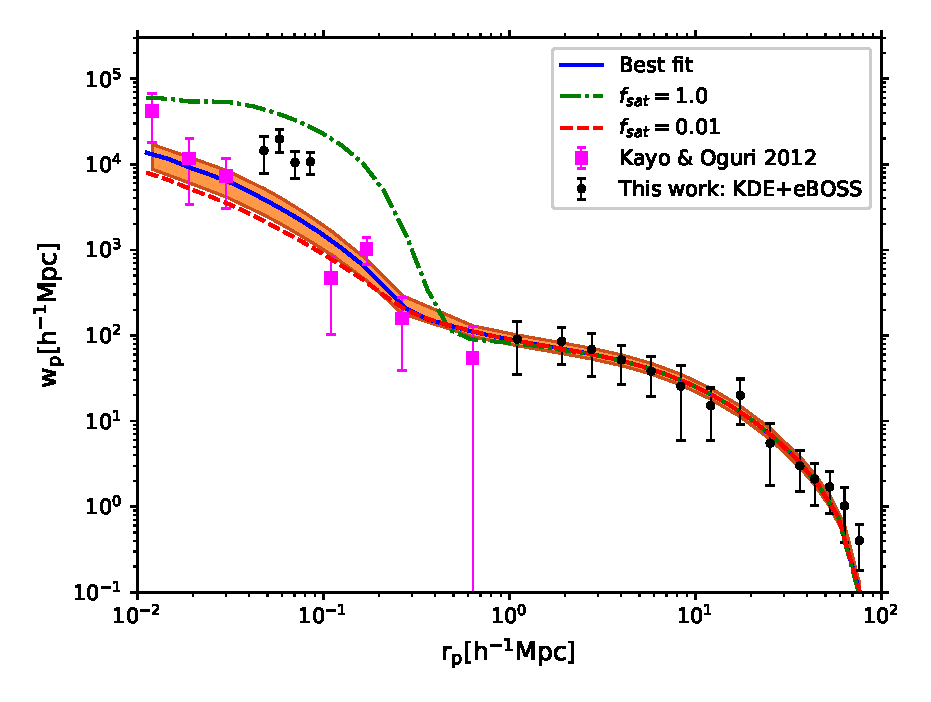
\includegraphics[angle=0,scale=0.6]{Bestfit_bestfit_2pars_4KDE.eps}
       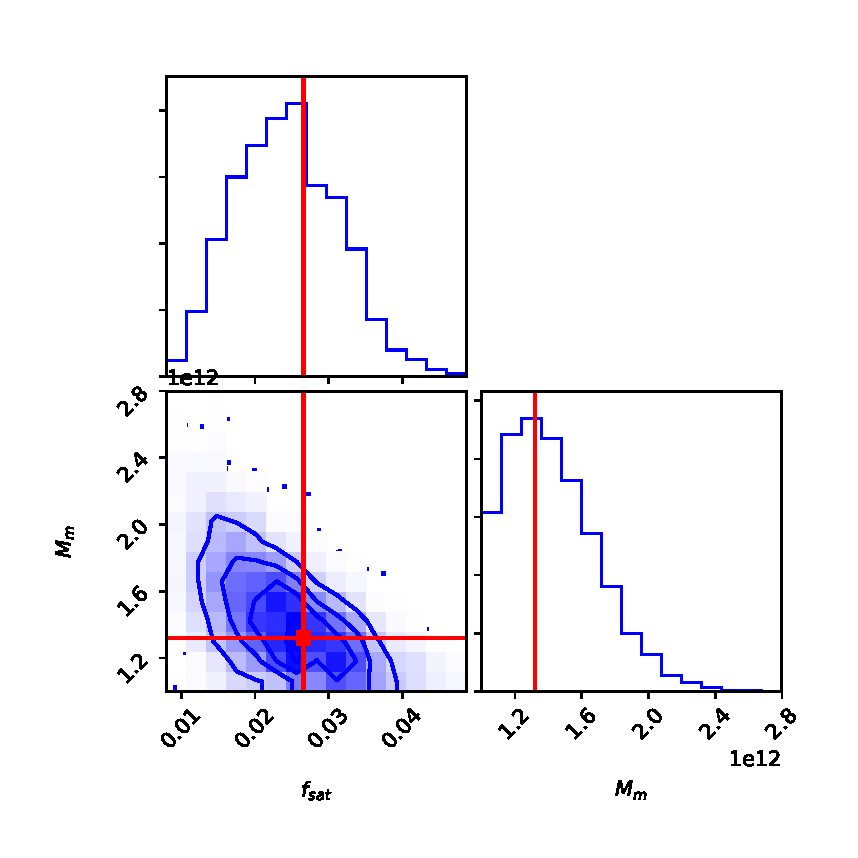
\includegraphics[angle=0,scale=0.6]{cornerplot_SEP18_4KDE.eps}}
    \caption{Left: Our HOD prediction of the projected correlation function that 
best-fits the observational data. The solid blue curve is the best-fit and the 
red dashed and green dotted-dashed lines are the model with best-fit $M_{m}$ but 
$f_{sat}=0.01$ and $f_{sat}=1.0$. We verified that relaxing $\Delta_{\rm m}$, as 
the third parameter, has no significant effect on the shape of the best-fit 
model. The best-fit value for $\Delta_{\rm m}$ stays consistent with 0.75 that 
was derived independently by KO12. The shaded envelope around the best 
fit model is the extent of the 2-sigma certainty for the shape of the HOD model 
at each bin of the projected distance ($\rm r_p$). All the data points depicted 
here (filled pink squares from KO12 and filled black circles) have 
participated in the fit. See $\S$\ref{dat} for a description of the clustering 
measurement from two separate sets of observations at $z \sim 1.5$ at small 
($\rm kpc$) and large ($\rm Mpc$) scales. Best fit model has $\rm M_{m} = 
1.43_{-0.23}^{+0.31} \times 10^{12}\, h^{-1} M_{\odot}$, and $f_{\rm sat} = 
0.0244_{-0.0070}^{+0.0075}$ with $\chi_{red}^{2} = 1.46$. Right: The result of 
the 2-parameter Monte-Carlo fit to the projected two point correlation function 
over $ \sim 0.01-100 \, \rm h^{-1} Mpc$ for the model shown in the left. 
Diagonal panels show the probability distribution functions (PDFs) of the 
fitting parameters (i.e., satellite fraction ($f_{sat}$), minimum halo mass that 
hosts a quasar ($M_{min}$), and the range of the halo masses that quasars occupy 
($\Delta_{m}$)). The off-diagonal panels show the density contours of the chosen 
sets of HOD parameters within one to three-sigma certainties. As the Marcov 
Chain explores the parameter space for each of the fitting parameters, each step 
of the chain takes a random walk with a randomly chosen step size and calculates 
the likelihood of the new set of parameters based on the difference between 
their deduced chi-squared and that of the previous set of chosen 
parameters.}\label{fig3:bfit}
    \end{subfigure}
\end{figure*}

\begin{figure*}
    \centering
        \begin{subfigure}{
        \centering
        \includegraphics[angle=0,scale=0.6]{Bestfit_wpmodel_2pars_1KDE.eps}
        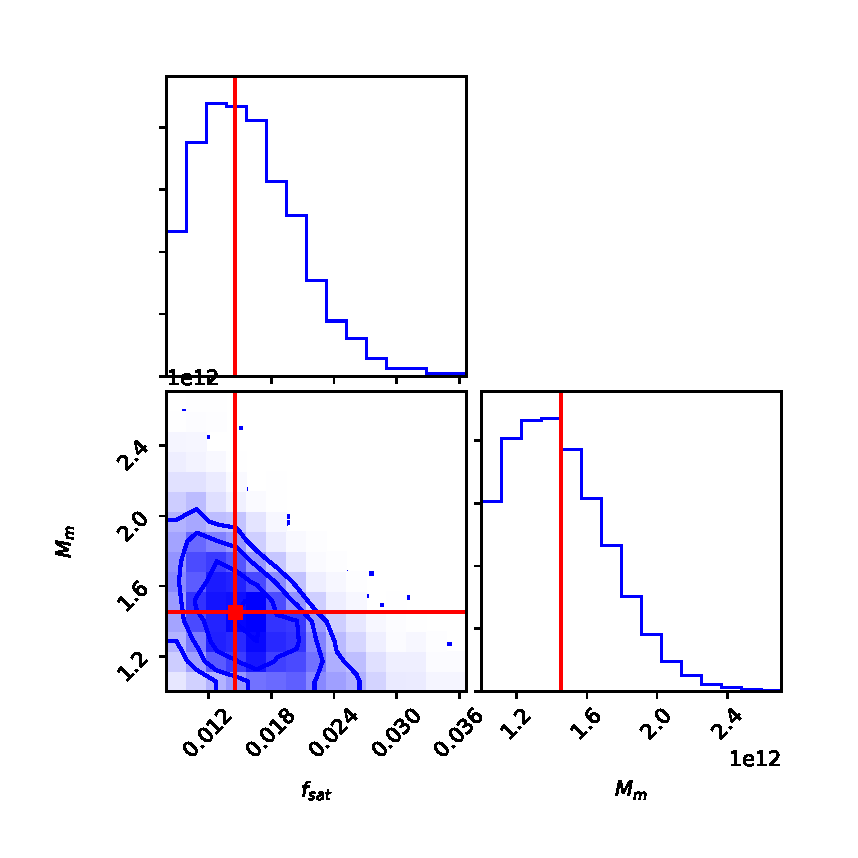
\includegraphics[angle=0,scale=0.6]{cornerplot_SEP18_ONLY1KDE.eps}}
        \caption{Left: Similar to the right panel of Fig.\,\ref{fig3:bfit} but 
for a single bin of the measured correlation function using the KDE-complete 
sample of close pairs. Best fit model(solid blue curve) has $\rm M_{m} = 
1.45_{-0.25}^{+0.32} \times 10^{12}\, h^{-1} M_{\odot}$, and $f_{\rm sat} = 
0.016_{-0.004}^{+0.005}$ with reduced $\chi^{2} = 1.18$. The shaded envelope 
around the best fit model is the extent of the 2-sigma certainty for the shape 
of the HOD model at each bin of the projected distance ($\rm r_p$). Right: 
Fitting statistics similar to the one shown for the fitting process in the 
right-hand panel of Fig.\,\ref{fig3:bfit}.}\label{fig4:cor}
       \end{subfigure}
\end{figure*}


% Modeling the Halo Occupation Distribution is essentially estimating the mean 
% number of quasars in individual haloes by modeling their distribution as a 
% function of a number physical parameters that characterize the interplay between 
% virialized dark matter overdensities and the embedded baryonic matter within 
% them.  
Following a commonly assumed mass-dependence, we model the mean number of 
occupying quasars in individual haloes simply by a three parameter Gaussian 
form: 

\begin{equation}
\langle N(M) \rangle = f_{N} \times \frac{1}{\sqrt{\left(2\pi \right)}\Delta_m} exp[-\frac{ln^2(M/M_m)}{2\Delta^{2}_m}],
\end{equation}

where $M_m$ is the minimum mass for a dark matter halo that can host a quasar 
and $\Delta_m$ is the width of the initial mass distribution. $f_N$ is the 
normalization factor that matches the observed number density of the quasars in 
our sample ($\sim6.462 \times 10^{-6} \, \rm h^3 Mpc^{-3}$) with its expected 
value from the halo mass function and the assumed distribution of haloes.
In the one-halo term of the power spectrum where the correlation function is 
measured with the pairs of haloes within boundaries of individual haloes 
themselves, there needs to be assumptions for the fraction of quasars that exist 
as ``satellite''s to a central quasar ($f_{sat}$) and the fraction of quasars 
that reside at the center of dark matter haloes ($p$). 
The halo occupation model then has ``central'' and ``satellite'' components such 
that $\langle N_{cen}(M)\rangle = (1-f_{sat})\langle N(M)\rangle$ and $\langle 
N_{sat}(M)\rangle = f_{sat} \langle N(M)\rangle$ \citep{bw02,kra04, zh05}.
KO12 justifies ignoring the mass dependence of the satellite fraction 
(i.e., $f_{sat}(M) \simeq f_{sat}$) by choosing a relatively narrow ($\sim 2$ 
dex) range for the halo mass distribution around the characterized minimum mass, 
$M_m$. Similar to their approach, we assume a constant satellite fraction and 
investigate any difference by relaxing the width of the halo mass distribution, 
$\Delta_m$, as an additional fitting parameter in our HOD model. 

We further adopt the ``independent quasar activity'' assumption for the central 
and satellite quasars that facilitates the use of Poisson statistics for the 
integrator in \citep{sel00}'s description of the one-halo term of the power 
spectrum \citep{ko12}:

 \begin{multline}
P_{1h}(k) = \frac{1}{n^{2}_{q}} \int \langle N(N-1)\rangle u(k,M)^p \frac{dn}{dM} dM  \\
\equiv 2 \langle N_{cen} N_{sat}\rangle u(k,M) + \langle N_{sat}(N_{sat}-1)\rangle |u(k,M)|^2 \\
%  
= [2 f_{sat}(1-f_{sat}) u(k,M)+f_{sat}^2 |u(k,M)|^2] \langle N(M)\rangle,
 \end{multline}

where $u(k,M)$ is the Fourier transform of the quasar number density profile in 
a dark matter halo of mass M. We adopt an NFW profile \citep{nfw97} with 
concentration parameter
\begin{equation}
c(M,z) = \frac{c_{0}}{1+z}[\frac{M}{M^{*}}]^{-0.13},
\end{equation}
 where $M^{*}$ is the nonlinear mass scale for collapse at $z=0$, $\beta = 
-0.13$ \citep{cs02}. In this work, we initially chose $c_0=9$ and investigated 
the change in the best-fit parameters for a model with haloes with 10 times 
higher concentration (see the right panel of Fig. \ref{fig5:10c}). A weak 
dependency of the HOD model to the concentration parameter is reported by a 
number of studies \citep{ric12,ric13,sh13} that used a different HOD formalism 
where the distribution of the central and satellite haloes are assumed to be a 
softened three-parameter step function and a two-parameter power-law 
respectively.
 We further discuss the differences between our chosen parameters and those 
previously used in the literature in $\S$\ref{res} where we summarize the 
differences between assumptions and their potential effect on the best-fit 
parameters.    

\section{Results and Discussion}\label{res}

We performed the fitting procedure of our constructed HOD model to the 
clustering measurement on a variety of data combinations including and excluding 
seven to 8 eight bins of the measured correlation function from KO12 (filled pink 
squares in Fig.\,\ref{fig3:bfit}, Fig.\,\ref{fig4:cor} and 
Fig.\,\ref{fig5:10c}). We justified the use of this measurement based on the 
close number density of the spectroscopic quasar sample used in their study 
($\sim1.35 \times 10^{-6} \, \rm h^3 Mpc^{-3}$), and the close average redshift 
of their sample ($z\sim1.4$). Assuming that quasars do not evolve rapidly in 
$\Delta z \sim 0.1$ time scale and the quasars in our KDE+eBOSS sample and those 
used by KO12 do not belong to different luminosity class ({\bf do we know 
this for a fact? KDE sample has targets down to i=23 but Kayo and Oguri 2012 
sample has quasars down to i=20}), we used a section of their measurement to fill 
the gap between our small and large scale measurements. We examined the effect 
of usnig the four binned correlation function or using the single-binned 
measurements in the best fit parameters (see Fig.\,\ref{fig3:bfit} and 
Fig.\,\ref{fig4:cor}). Table\,\ref{tab:res} summarizes the fitting results for 
all the fitting trials. 
\begin{figure*}
    \centering
    \begin{subfigure}{
     \centering
       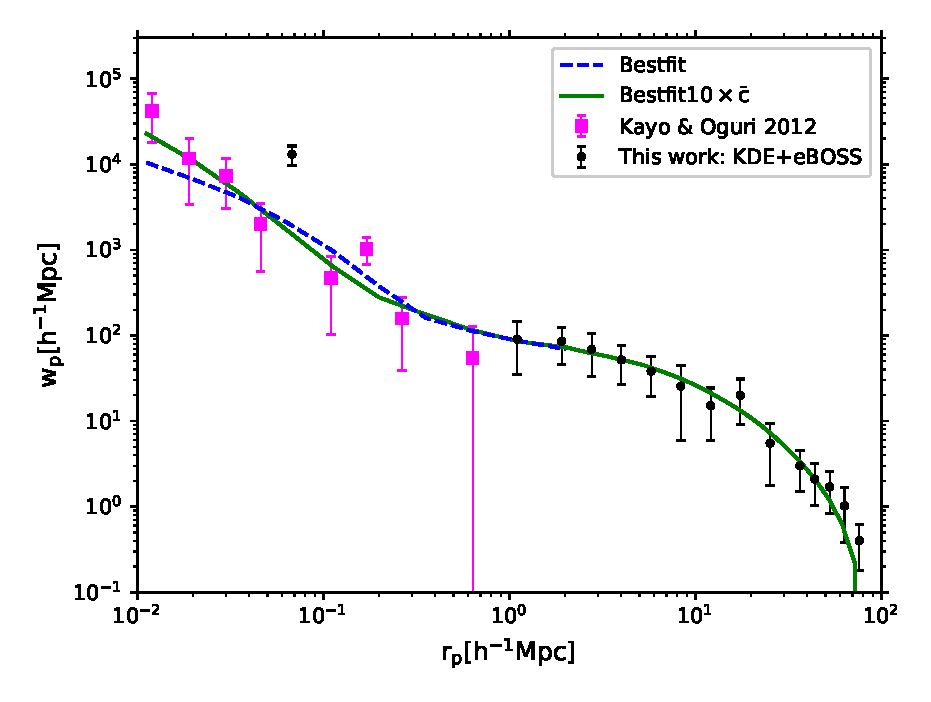
\includegraphics[angle=0,scale=0.6]{Bestfit_with_wp10c_2pars_1KDE.eps}
       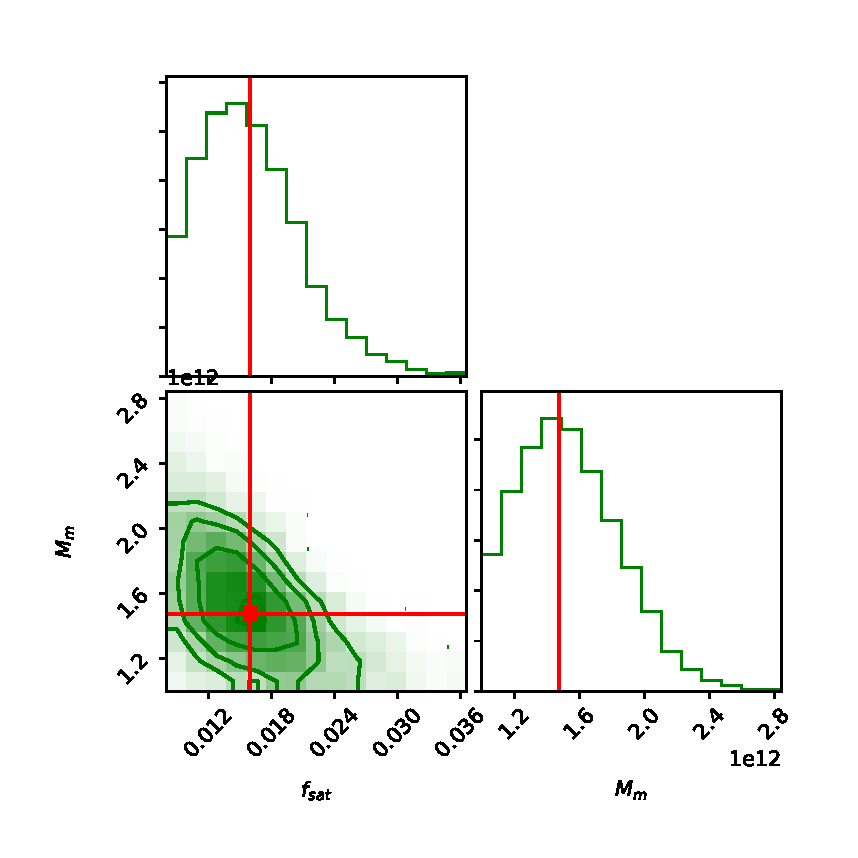
\includegraphics[angle=0,scale=0.6]{cornerplot_SEP18_1KDE_10c.eps}}
    \caption{Left: Our HOD prediction of the projected 
correlation function that best-fits the full-scale measurement (all the shown 
data points participated in the best-fit determination) and where the dark 
matter haloes are assumed to have 10 times higher average concentrations than the 
best-fit model shown with the dashed blue line (solid blue curve in 
Fig.\ref{fig4:cor}). The best-fit model (solid green line) has $\rm M_{m} = 
1.55_{-0.29}^{+0.35} \times 10^{12}\, h^{-1} M_{\odot}$, and $f_{\rm sat} = 
0.016_{-0.004}^{+0.005}$ with reduced $\chi^{2} = 1.213$. The shaded envelope 
around the best-fit model is the extent of the 2-sigma certainty for the shape 
of the HOD model at each bin of the projected distance ($\rm r_p$). Although the 
steeper shape of the one-halo term seems to better follow the measurements 
reported in small scales, the fitting results do not show a significantly better 
constraint on the fitting parameters.}\label{fig5:10c}
    \end{subfigure}
\end{figure*}


Influenced by the parameterization used in KO12, we investigated 
relaxing $\Delta_{\rm m}$ as the third parameter for the HOD model (in addition 
to $f_{\rm sat}$ and $\rm M_{m}$) and found it to have no significant effect in 
the best-fit model. We also examined the best-fit quality of an HOD model with 
10 times higher average concentration parameter ($10 \times \bar c$) to the full-scale 
correlation function (with and without inclusion of KO12's measurement 
in the fit). Figure\,\ref{fig5:10c} shows a steeper one-halo term 
for the best-fit model that is more in accord with the measured correlation function by 
KO12. But this {\it shape change} has not led to inconsistent best-fit parameters with those of the 
best-fit model with haloes of normal concentration (see the second and the third rows of Table\,\ref{tab:res}). 

To remove the added assumptions for including past measurements in the results, we fit the same two-parameter HOD model used in prior fitting processes only to our measured $w_p$ from the KDE-complete sample of close pairs and our Mpc-scale measurement from the eBOSS sample, leaving KO12 measurement out of the fitting procedure. The solid blue line in Figure \,\ref{fig6:kdeboss} represents the best-fit to this data (KDE+eBOSS). The solid dark red model is the best-fit model to the same KDE+eBOSS measurements but also the measured $w_p$ over eight bins of comoving distance from KO12. The shaded envelopes that represent the 1-$\sigma$ uncertainties for the best-fit models, are visibly separated. This indicates that inclusion of the clustering measurement at $z\sim1.4$ results in a significantly different best-fit (see the second and the last row of Table\,\ref{tab:res}). The lower clustering signal measured for quasars in KO12 sample results in $> \times 30$ smaller satellite fraction compared to what KDE clustering alone implies. However, our best-fit $f_{sat}= 0.062_{-0.026}^{+0.028}$ is consistent with KO12 report of $f_{sat}= 0.048_{-0.015}^{+0.016}$ with $\chi_{red}^2 = 0.89$ for an NFW profile. 
%KO12 found that dark matter haloes with the {\it peak mass} of $\rm M_m=1.33_{-0.32}^{+0.36}\times 10^{13}\, h^{-1} M_{\odot}$

\begin{table*}
\centering
\begin{tabular}{lccc}

\hline
\hline
Data &$\rm M_m (\times 10^{12}\, h^{-1} M_{\odot})$ &$f_{sat}$& $\chi_{red}^2$ (d.o.f)\\
\hline
 \vspace{.1in}
 4KDE+14eBOSS+7KO12& $1.43_{-0.25}^{+0.31}$& $0.024_{-0.007}^{+0.007}$& 1.460 (22)\\
 \vspace{.1in}
 1KDE+14eBOSS+8KO12& $1.45_{-0.25}^{+0.32}$& $0.016_{-0.004}^{+0.005}$& 1.180 (20)\\
 \vspace{.1in}
 1KDE+14eBOSS+8KO12 ($10\times \bar c$)& $1.55_{-0.29}^{+0.35}$& $0.016_{-0.004}^{+0.005}$& 1.213 (20)\\
 \vspace{.1in}
 1KDE+14eBOSS & $2.32_{-0.44}^{+0.46}$& $0.062_{-0.026}^{+0.028}$& 0.855 (12)\\

\hline
\end{tabular}
\caption{ Summary of the fitting results using different data that participated in 
the fit. The second and third columns are the best-fit parameters and their 1-$\sigma$ uncertainties. The last column lists the reduced 
$\chi^2$ (and the degrees of freedom). }\label{tab:res}
\end{table*}

Recent HOD analysis of the local AGNs at $z \sim 0.01-0.1$ has revealed that 
AGNs reside in similar dark matter haloes to that of galaxies with similar 
stellar mass (reference a recent analysis with BASS-2MASS CCF measurement at 
z=0.01-0.1 using HALOTOOLS package). 
This could be interpreted as a by product of observing no significant luminosity 
dependency of quasar and AGN clustering,  

A look at the recent investigations on the effective environmental factors that 
lead to presence of two AGN types and the contradictory findings on the 
difference between their bias with respect to dark matter, halo mass, black hole 
mass, mean number of satellites \citep[see, e.g.,][]{Dip14CMB,Dip17a,kr18} is a 
shining evidence of the need for theoretical followup and pairing up the 
measured correlation function with complementary measurements that enhances the 
presence of the observationally challenging bins at kpc scales \citep[see, ][for 
a proposed alternative]{sta11}. 

In recent years, an increasing number of reports on the persistent degeneracies 
between the best-fit parameters of widely used HOD formalism (initially 
designed for local AGNs) have emerged \citep{Coi16,coi17}. 


\begin{figure}
    \centering
    %\begin{subfigure}{
     %\centering
       \includegraphics[angle=0,scale=0.6]{Bestfit_2pars_1KDE_NOKO12.eps}
      % \includegraphics[angle=0,scale=0.6]{cornerplot__1KDE_NOKO12.eps}}
    \caption{Left: Our HOD prediction of the projected correlation function that 
best-fits the full-scale measurement where only the measurement from 
KDE-complete sample of close pairs and the data from eBOSS clustering is added 
(solid blue curve in Fig.\ref{fig4:cor}). The best-fit model
has $\rm M_{m} = 2.32_{-0.440}^{+0.463} \times 10^{12}\, h^{-1} M_{\odot}$, and 
$f_{\rm sat} = 0.062_{-0.026}^{+0.028}$ with reduced $\chi^{2} = 1.09$. The 
shaded envelope around the best-fit model is the extent of the 1-sigma certainty 
for the shape of the HOD model at each bin of the projected distance ($\rm 
r_p$). }\label{fig6:kdeboss}
  %  \end{subfigure}
\end{figure}



 These studies differ from this work (as well as KO12) in two 
significant ways: (i) The two-point correlation function in those studies fall 
short of measurements over scales well within individual halo ($\sim 10-100 \, 
\rm h^{-1} kpc$ ) where the one-halo term of the power spectrum has an ideal 
chance of constraining with observation at those scales. (ii) We assumed a 
Gaussian form for distribution of both central and satellite haloes (add an 
argument for what this assumption terms of the assembly history). \citet{sh13} 
performed a comprehensive investigation of the formalism introduced by 
\citet{zh05} and implemented by a number of clustering analysis ever since 
\citep{zh07,mi11,zeh11,ric12,ric13}(add more refs) by performing a five and six 
parameter fit to their galaxy-quasar cross correlation function at $\bar z \sim 
0.5$  
 
\section*{Acknowledgments}
SE and ADM acknowledge support by the National Science Foundation (NSF) through the 
grant number 10 times. 

Funding for the Sloan Digital Sky Survey IV has been provided by the Alfred P. 
Sloan Foundation, the U.S. Department of Energy Office of Science, and the 
Participating Institutions. SDSS acknowledges support and resources from the 
Center for High-Performance Computing at the University of Utah. The SDSS web 
site is \url{http://www.sdss.org}.

SDSS is managed by the Astrophysical Research Consortium for the Participating 
Institutions of the SDSS Collaboration including the Brazilian Participation 
Group, the Carnegie Institution for Science, Carnegie Mellon University, the 
Chilean Participation Group, the French Participation Group, Harvard-Smithsonian 
Center for Astrophysics, Instituto de Astrof\'{i}sica de Canarias, The Johns 
Hopkins University, Kavli Institute for the Physics and Mathematics of the 
Universe (IPMU) / University of Tokyo, Lawrence Berkeley National Laboratory, 
Leibniz Institut f\"{u}r Astrophysik Potsdam (AIP), Max-Planck-Institut f\"{u}r 
Astronomie (MPIA Heidelberg), Max-Planck-Institut f\"{u}r Astrophysik (MPA 
Garching), Max-Planck-Institut für Extraterrestrische Physik (MPE), National 
Astronomical Observatories of China, New Mexico State University, New York 
University, University of Notre Dame, Observatório Nacional / MCTI, The Ohio 
State University, Pennsylvania State University, Shanghai Astronomical 
Observatory, United Kingdom Participation Group, Universidad Nacional 
Aut\'{o}noma de M\'{e}xico, University of Arizona, University of Colorado 
Boulder, University of Oxford, University of Portsmouth, University of Utah, 
University of Virginia, University of Washington, University of Wisconsin, 
Vanderbilt University, and Yale University.
\newpage
\bibliographystyle{mn2e.bst}
\bibliography{hodrefs}
\end{document}
